\section{Program flowchart}
\label{chapter3}


\paragraph{}
\ref{fig:stateDiagrams} shows the state transition diagrams for Node 1 and Node 2. Both nodes execute a thread that sets up the Bluetooth communication and sends and receives data. Node 1 executes a second thread which periodically fetches the proximity sensor readings, and provides them to the communication thread for transmission to Node 2. Node 2 executes a thread which uses the current speed and distance data to automatically control the vehicle speed if the ACC system is turned on.

\begin{figure}[h]
	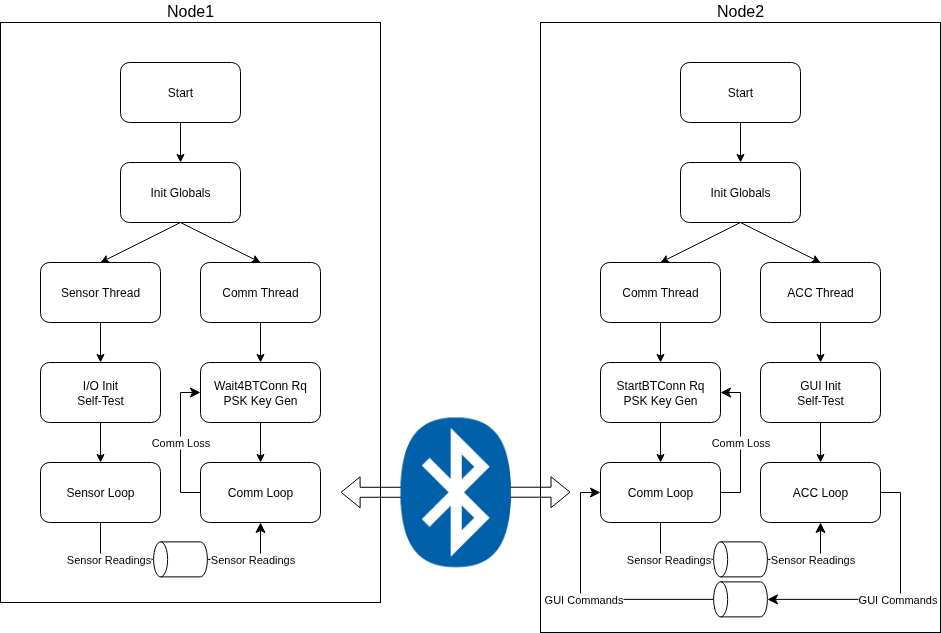
\includegraphics[height=100mm]{images/StateDiagrams.png}
	\centering
	\caption{State Diagrams}
	\label{fig:stateDiagrams}
\end{figure}

\paragraph{}
\ref{fig:stateDiagramNode1} shows the two thread loops of Node 1 in more detail. The Sensor Loop sequentially obtains readings from the two connected sensors, checks the value for plausibility and consistency. Depending on whether values are OK, the thread pushes the normalized distance data or an error code to a global variable, where the communication thread picks it up for further transmission. In the end, the thread is put to sleep for a short amount of time after which it starts over.

\paragraph{}
The communication loop waits for request messages to be received. If an error happens during data reception, the Bluetooth connection is closed and a new one is set up. On successful message reception, the data is parsed and checked for authenticity and validity (i.e. the MAC and counter values are verified for correctness). Requests which fail these checks are ignored. If the received message turns out to be a request for a transmission of the distance readings, the thread picks up the distance data from a global variable and puts it into a message which it transmits to Node 2. If the transmission fails, the Bluetooth transmission is closed again and a new one is set up. On successful transmission, the thread puts itself to sleep for a short amount of time after which it starts over.

\paragraph{}
The steps in diagram \ref{fig:stateDiagramNode1} which are drawn in inverted color involve read or write operations on shared global data. In order to avoid race conditions the read/write operations are protected in critical sections.

\begin{figure}[h]
	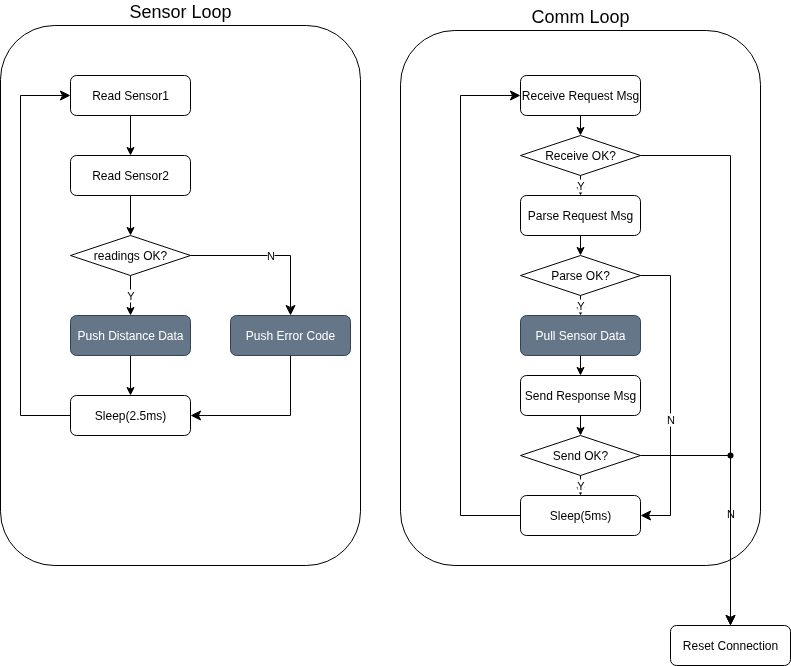
\includegraphics[height=100mm]{images/StateDiagramNode1.png}
	\centering
	\caption{State Diagrams Node 1}
	\label{fig:stateDiagramNode1}
\end{figure}

\paragraph{}
\ref{fig:stateDiagramNode2} shows the two thread loops that execute on Node 2. The communication loop sends a request message for a new distance reading value to Node 1. If the response message passes the authenticity and validity checks, the received sensor data is copied into a global variable where it can be picked up from the ACC thread. In the last step the thread puts itself to sleep for a short amount of time, after which it starts over. Similar to Node 1, if either message reception or transmission fails, the current connection is closed and a new one is set up. Received messages which fail authenticity and validity checks are ignored.

\paragraph{}
The ACC loop retrieves from the GUI the ACC status (whether the driver has turned it on or off) and, if it is turned off, the current, manually set, speed. In the next step, it obtains the Sensor data (i.e. the most recently received distance data). It verifies whether an error code or a valid distance was received, and also whether the age counter of the reading lies within the allowed threshold. If either age or value indicate an error, an error counter is incremented. If the error counter is above a given threshold of four incorrect readings, the state of the ACC is set to ERROR. If the error counter lies below that threshold the distance reading is ignored (and the last successful distance is used in the subsequent steps instead). If both value and age of the reading are OK, the reading is accepted as current distance, moreover the state of the ACC is set to OFF if it was previously in the ERROR state.
In the next step, if ACC is in the ON state, a control function \emph{Speed = ACC(Distance, Speed)} is applied, i.e. the ACC accelerates/decelerates the car depending on the current vehicle speed and measured distance.
Thereafter, the current vehicle speed, distance, and ACC state is conveyed to the display so it can update the corresponding GUI elements. In the last step, the control loop puts itself to sleep for a short amount of time and thereafter starts over. Like in the previous diagram, steps in inverted color indicate read/write accesses to data shared across threads. These accesses are protcted by critical sections.

\begin{figure}[h]
	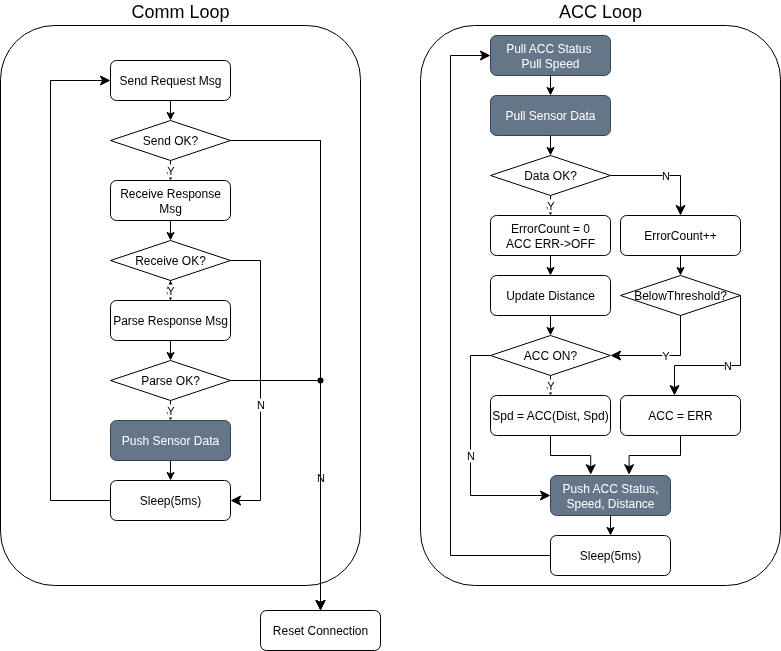
\includegraphics[height=100mm]{images/StateDiagramNode2.png}
	\centering
	\caption{State Diagrams Node 2}
	\label{fig:stateDiagramNode2}
\end{figure}
